\providecommand{\pgfsyspdfmark}[3]{}
\providecommand{\savepicturepage}[3]{}

\documentclass[11pt,letterpaper]{article}
\usepackage[lmargin=1in,rmargin=1in,tmargin=1in,bmargin=1in]{geometry}

% -------------------
% Packages
% -------------------
\usepackage{
	amsmath,			% Math Environments
	amssymb,			% Extended Symbols
	enumerate,		    % Enumerate Environments
	graphicx,			% Include Images
	lastpage,			% Reference Lastpage
	multicol,			% Use Multi-columns
	multirow,			% Use Multi-rows
	gensymb
}


% -------------------
% Font
% -------------------
\usepackage[T1]{fontenc}
\usepackage{charter}


% -------------------
% Commands
% -------------------

\newcommand{\prob}{\noindent\textbf{Problem. }}
\newcounter{problem}
\newcommand{\problem}{
	\stepcounter{problem}%
	\noindent \textbf{Problem \theproblem. }%
}
\newcommand{\pspace}{\par\vspace{\baselineskip}}
\newcommand{\ds}{\displaystyle}


% -------------------
% Header & Footer
% -------------------
\usepackage{fancyhdr}

\fancypagestyle{pages}{
	%Headers
	\fancyhead[L]{}
	\fancyhead[C]{}
	\fancyhead[R]{}
\renewcommand{\headrulewidth}{0pt}
	%Footers
	\fancyfoot[L]{}
	\fancyfoot[C]{}
	\fancyfoot[R]{}
\renewcommand{\footrulewidth}{0.0pt}
}
\headheight=0pt
\footskip=14pt

\pagestyle{pages}


% -------------------
% Content
% -------------------
\begin{document}
\noindent\textbf{\large Calculus II (MSF\_10010 / AM\_\_1080AH) \\ 2023 Spring \\ Problem List IX (Due May 4)}

\bigskip

\noindent\begin{minipage}{0.7\textwidth}
    \problem The equation of an ellipse with its long axis placed on the $x$-axis and short axis placed on the $y$-axis, shown on the right, is
\[\frac{x^2}{a^2}+\frac{y^2}{b^2} = 1\]
where $a$ and $b$ are half the lengths of its long and short axes.  Base on this equation, show that the area of the ellipse is $\pi a b$.
\end{minipage}
\begin{minipage}{0.3\textwidth}
    \begin{center}
        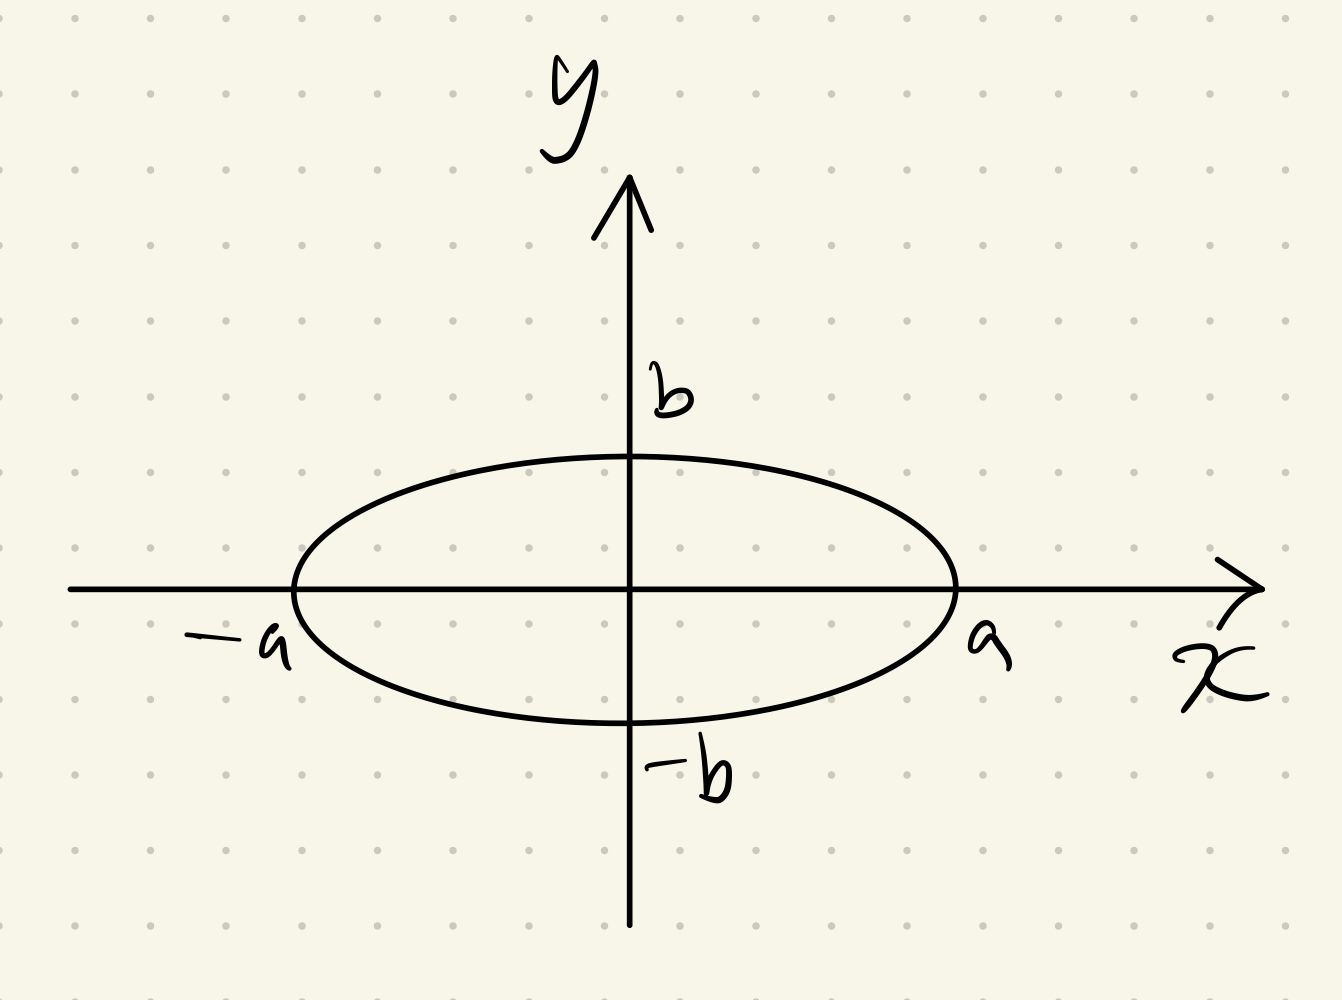
\includegraphics[width = 0.9\textwidth]{../graph/A09.png}
    \end{center}
\end{minipage}
\vspace{15mm}

\problem Find the area enclosed by $y = \frac{3}{2}\tan x$, $y = \cos x$ and the $y$-axis on a Cartesian plane.
\vspace{15mm}

\problem Find the area between $y = \ln x$ and $y = 0$ from $x = \frac{1}{2}$ to $2$ on a Cartesian plane.
\vspace{15mm}

\problem Find the arc length of $y = \ln x$ from $x = 1$ to $\sqrt{3}$ on a Cartesian plane.  

\noindent (Hint: Use trigonometric substitution first, transform the integrand into sines and cosines, then use U-substitution on one of sine and cosine.)
\end{document}